

\documentclass[a4paper,12pt]{report}

% --- 0 nome appunti


% --- 1. LINGUA E FONT ---
\usepackage[T1]{fontenc}
\usepackage[utf8]{inputenc}
\usepackage[italian]{babel} % Traduce "Chapter" in "Capitolo", ecc.
\usepackage{lmodern}        % Font vettoriale di alta qualità
\usepackage{ulem}
\usepackage{multirow}
\usepackage{makecell}

% --- 2. GEOMETRIA E IMPAGINAZIONE ---
\usepackage[a4paper, top=2.5cm, bottom=2.5cm, left=2.5cm, right=2.5cm]{geometry}
\usepackage{titlesec}       % Personalizzazione dei titoli
\setlength{\parindent}{0pt}
% Rimuove la scritta "Capitolo X" e affianca il numero al titolo
\titleformat{\chapter}[hang]
  {\normalfont\huge\bfseries}{\thechapter.}{20pt}{\Huge}
\titlespacing*{\chapter}{0pt}{-20pt}{30pt}

% --- 3. MATEMATICA E SIMBOLI ---
\usepackage{amsmath, amssymb, amsfonts}

% --- 4. GRAFICA E IMMAGINI ---
\usepackage{graphicx}
\usepackage{float}          % Permette l'uso di [H] per forzare la posizione delle immagini
\usepackage{caption}        % Personalizzazione delle didascalie
\usepackage{subcaption}     % Per affiancare più immagini
\usepackage{geometry}
\geometry{a4paper, margin=1.25cm}
\usepackage{parskip}
\usepackage{titlesec}
\usepackage{xltabular}

% --- 5. TIKZ ---
\usepackage{tikz}

% --- 6. LISTE E TABELLE ---
\usepackage{enumitem}       % Controllo avanzato di itemize e enumerate
\usepackage{booktabs}       % Tabelle professionali (toprule, midrule, bottomrule)
\usepackage{tabularx}       % Tabelle che si adattano alla larghezza della pagina

% --- 7. FORMATTAZIONE DEL CODICE (LISTINGS) ---
\usepackage{listings}
\usepackage{xcolor}

% Definizione colori per il codice
\definecolor{codegreen}{rgb}{0,0.6,0}
\definecolor{codegray}{rgb}{0.5,0.5,0.5}
\definecolor{codepurple}{rgb}{0.58,0,0.82}
\definecolor{backcolour}{rgb}{0.95,0.95,0.92}

% Configurazione stile codice (ottimizzato per Java/C++)
\lstdefinestyle{oopstyle}{
    backgroundcolor=\color{backcolour},   
    commentstyle=\color{codegreen}\itshape,
    keywordstyle=\color{magenta}\bfseries,
    numberstyle=\tiny\color{codegray},
    stringstyle=\color{codepurple},
    basicstyle=\ttfamily\footnotesize,
    breakatwhitespace=false,         
    breaklines=true,                 
    captionpos=b,                    
    keepspaces=true,                 
    numbers=left,                    
    numbersep=5pt,                  
    showspaces=false,                
    showstringspaces=false,
    showtabs=false,                  
    tabsize=2,
    frame=single,
    rulecolor=\color{black!30}
}
\lstset{style=oopstyle}

% --- 8. BOX COLORATI (PATTERN GRASP, GOF, PROCESSO UP) ---
\usepackage[most]{tcolorbox}

% --- 9. COLLEGAMENTI E INDICE (Da caricare per ultimo) ---
\usepackage{hyperref}
\hypersetup{
    colorlinks=true,
    linkcolor=blue!70!black, % Colore dei link interni (indice)
    filecolor=magenta,       % Colore dei link a file
    urlcolor=cyan,           % Colore degli URL
    pdftitle={Appunti di Ricerca Operativa e Pianificazione delle Risorse},
    pdfauthor={Nicholas Scorrano},
    pdfpagemode=UseOutlines
}
\usepackage{bookmark} % Migliora i segnalibri nel lettore PDF
\usepackage{caption}
\usepackage{multirow}
\usepackage{graphicx}
\usepackage{amsmath}
\usepackage{nicematrix}
\usepackage{tikz}

\begin{document}

    \begin{titlepage}
        \centering
        
        \begin{center}
            
\includegraphics{Immagini/Logo Bicocca.png}
        \end{center}
        
        \vspace{2cm}
        
        {\Huge \textbf{Appunti di Ricerca Operativa e Pianificazione delle Risorse}}
        
        \vspace{1.5cm}
        
        {\Large Nicholas Scorrano} % Inserisci qui il tuo nome
        
        \vspace{1.5cm}
        
        {\Large Anno Accademico 2026/2027}

        \vspace{1.5cm}

        {
            \Large
            \textbf{Discalimer}:


            Questi sono miei appunti personali, potrebbero contenere inesattezze
        }
    \end{titlepage}

    \tableofcontents

    \setcounter{part}{-1}
    \part{Prerequisiti}

    \part{Teoria}
        \setcounter{chapter}{-1}
        \chapter{Introduzione alla Ricerca Operativa}
\section{Cosa è la Ricerca Operativa?}
La ricerca operativa è la disciplina che si occupa della ricerca nelle operazioni.

La ricerca operativaè, quindi, applicata a problemi di gestione e di coordinamento delle attività nell'ambito di un'organizzazione

\subsection{Significato di "ricerca"}
La parola "ricerca" nel nome evidenzia il fatto che questa disciplina adotta lo stesso approccio usato negli altri campi scientifici.

Infatti, il metodo scientifico è usato, in larga misura, come metodologia di indagine per il problema in esame.

In particolare, il processo inizia con'accurata osservazione e formulazione del problema e la raccolta di tutti i dati relativo.

\section{I modelli nella ricerca operativoa}
Le fasi tipiche di uno studio di ricerca operativa possono essere riassunte in questo modo:
\begin{enumerate}
    \item Definizione del problema e raccolata dei dati
    \item Formulazione del modello matematico
    \item Determinazione delle soluzioni del modello
    \item Test e validazione del modello
    \item Predisposizione di un sistema di supporto all'applicazione del modello
    \item Implementazione del sistema
\end{enumerate}
        \chapter{Modelli nella ricerca operativa}
\section{Problemi di ottimizzazione}
\subsection{Definizione funzione obiettivo e della formulazione del problema di ottimizzazione}
Data una funzione:
$$
    f:\mathbb{R}^n \to \mathbb{R} \longrightarrow \text{\textbf{Definita come \uline{funzione obiettivo}}}
$$

Un \textbf{problema di ottimizzazione} è formulabile come segue:
$$
    \begin{aligned}
        & \text{opt} & & f(x)  \\
        & \text{s.a.} & & x \in X \quad X \subseteq \mathbb{R}^n
    \end{aligned}
$$

$\mathbf{opt}$ è un \uline{operatore nella formulazione matematica generale} di un problema di ottimizzazione, viene usato per indicare l'operazione che si intende effettuare sulla funzione obiettivo, $opt \in \{min,max\}$

\subsection{Regione ammissibile}
X è detta regione ammissibile, cioè l'insieme delle soluzioni $x$ ammissibili dal problema.

\begin{minipage}[c]{0.45\textwidth}
    \vspace{0pt}
    \begin{itemize}
        \item Se $\mathbf{opt=min}$ abbiamo un \uline{problema di minimizzazione}
        \item Se $\mathbf{opt=max}$ abbiamo un \uline{problema di massimizzazione}
    \end{itemize}
\end{minipage}
\hfill
\begin{minipage}[c]{0.45\textwidth}
    \vspace{0pt}
    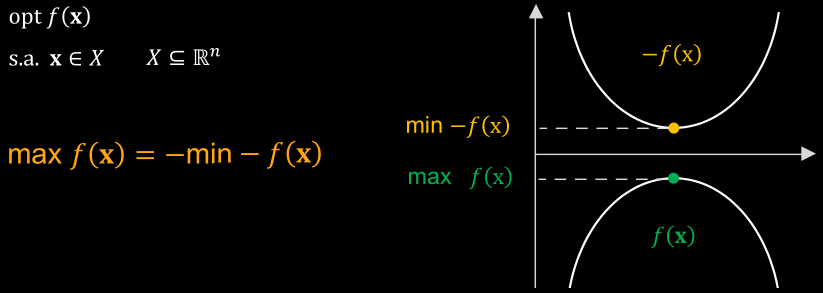
\includegraphics[width=\textwidth]{Immagini/minimizzazione-massimizzazione.png}
\end{minipage}

Le variabili che indicano i vincoli ai quali è soggetto il problema sono dette \textbf{variabili decisionali} e indentificano una soluzione del problema

\begin{minipage}[t]{0.45\textwidth}
    \subsubsection{Problema di massimizzazione}
    $$
    \begin{aligned}
        & \max f(x) & \longrightarrow \ & opt = \max \\
        & s.a. \ x \in X & \longrightarrow \ & \parbox[t]{5cm}{ \textbf{Variabili numeriche} in cui i valori identificano una soluzione del problema} \\
        & X \subseteq \mathbb{R}^n & \longrightarrow & \parbox[t]{5cm}{\textbf{Regione ammissibile}, ossia l'insieme delle soluzioni $x$ ammesse}
    \end{aligned}
    $$
\end{minipage}
\hfill
\begin{minipage}[t]{0.45\textwidth}
    \subsubsection{Problema di minimizzazione}
    $$
    \begin{aligned}
        & \min f(x) & \longrightarrow \ & opt = \max \\
        & s.a. \ x \in X & \longrightarrow \ & \parbox[t]{5cm}{ \textbf{Variabili numeriche} in cui i valori identificano una soluzione del problema} \\
        & X \subseteq \mathbb{R}^n & \longrightarrow & \parbox[t]{5cm}{\textbf{Regione ammissibile}, ossia l'insieme delle soluzioni $x$ ammesse}
    \end{aligned}
    $$
\end{minipage}

\subsection{In cosa consiste un problema di ottimizzazione?}
Un problema di ottimizzazione consiste nel determinare, se esistono, uno o più punti di $\min/\max\ \mathbf{x^*}$, assegnazioni di valori alle variabili decisionali $x$, della funzione obiettivo $f$ tra i punti $x \in X$

\newpage
\section{Tipologie di Ottimizzazione}
Quando parliamo di ottimizzazione di una funzione obiettivo possiamo avere diversi tipi di ottimizzazione

\subsection{Ottimizzazione NON vincolata}
La ricerca del/i punto/i di ottimo della funzione obiettivo viene condatta su tutto lo spazio di definizione della/e variabile/i di decisione

\begin{center}
    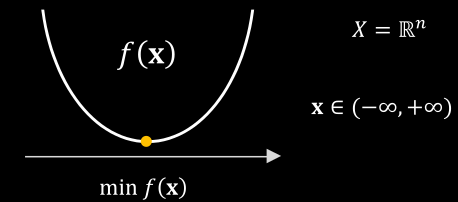
\includegraphics[scale=0.5]{Immagini/ott. non vincolata.png}
\end{center}


\subsection{Ottimizzazione vincolata}
La ricerca del/i punto di ottima della funzione obiettivo viene condotta su un sottoinsieme proprio dello spazio di definizione della/e variabile/i di decisione

\begin{center}
    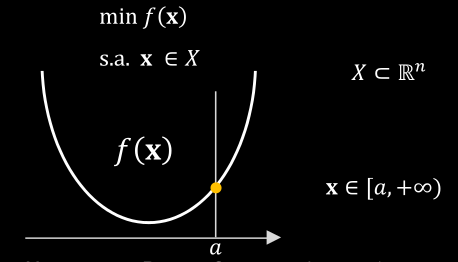
\includegraphics[scale=0.5]{Immagini/ott. vincolata.png}
\end{center}

\subsection{Ottimizzazione intera}
Le variabili assumono solo valori interi


{   \large
    $$
        \begin{aligned}
            opt f(x) \\
            s.a x \in X \\
            X \in \mathbb{Z}^n
        \end{aligned}
    $$
}

\subsection{Ottimizzazione binaria}
Le variabili assumono solo valore 0 o 1
{
    \large
    $$
        x \in \{0,1\}^n
    $$
}
\subsection{Ottimizzazione mista}
Alcune variabili assumono valori interni mentre altre variabili assumono solo valori binari.

Se non specifato altrimenti, si intende $X \subseteq \mathbb{R}^n$

\section{Programmazione Matematica}
\subsection{Definizione}
Quando l'insieme $X$ delle soluzioni ammissibili di un problema di ottimizzazione \uline{viene espresso attraverso un sistema di equazioni e disequazioni}, esso prende il nome di problema di \textbf{Programmazione Matematica}.

\subsection{Vincoli}
Un vincolo è un espressione del tipo


\begin{minipage}[c]{0.4\textwidth}
    {
    \large
    $$
        g_i(\mathbf{x})
        \left\{
        \begin{matrix}
        \geq \\
        = \\
        \leq
        \end{matrix}
        \right\}
        0
    $$
}
\end{minipage}
\hfil
\begin{minipage}[c]{0.4\textwidth}
    Dove intendiamo che $g_i(x)$ possa essere:
    \begin{itemize}
        \item $g_i(x) \geq 0$
        \item $g_i(x) = 0$
        \item $g_i \leq 0$
    \end{itemize}
\end{minipage}

Con $g_i:X \to \mathbb{R}$ funzione generica che lega tra loro le variabili decisionali.

In generale possiamo avere uno o più vincoli

\subsection{Definizione di Regione ammissibile (PM)}
La regione ammissibile è definita dall'insieme dei vincoli del problema

{
    \large
    $$
        X = \{x \in \mathbb{R}^n \text{ con } g_i(\mathbf{x})
        \left\{
        \begin{matrix}
        \geq \\
        = \\
        \leq
        \end{matrix}
        \right\}
        \ i=1,\dots,m
        \}   
    $$
}

Osserivamo, quindi, che abbiamo $m$ vincoli ed $n$ variabili
\begin{itemize}
    \item Se $\mathbf{x \in X}$ allora $x$ è \textbf{soluzione ammissibile}
    \item Se $\mathbf{x \not \in X}$ allora $x$ \textbf{non è una soluzione ammissibile}
\end{itemize}

\subsection{Tipologie di Regioni Ammissibili}

\subsubsection{Problema non ammissibile}
{
    \large

    $$
        X = \emptyset
    $$
}
Regione ammissibile vuota, nessuna soluzione ammissibile, problema mal posto

\subsubsection{Problema illimitato}
\begin{gather*}
    \forall c \in \mathbb{R},\ \exists x_C \in X : f(x_C) \leq c \quad \text{se } opt = min \quad \text{illimitato inferiormente} \\
    \forall c \in \mathbb{R},\ \exists x_C \in X : f(x_C) \geq c \quad \text{se } opt = min \quad \text{illimitato superiormente}
\end{gather*}

\subsubsection{Problema con soluzione ottima unica}

\subsubsection{Problema con più di una soluzione ottima (anche infinite)}
Tutte le soluzioni ottime hanno egual valore della funzione obiettivo

\newpage
\section{Ottimi globali e locali}

\subsection{Definizione Ottimo Globale}
La risoluzione di un problema di Programmazione Matematica consiste nel trovare una soluzione ammissibile che sia un \textbf{ottimo globale}, vale a dire un vettore $x^* \in X$ tale che :

\begin{gather*}
    f(x^*) \leq f(x) \quad \forall x \in X \quad \text{se } opt = min \\
    f(x^*) \geq f(x) \quad \forall x \in X \quad \text{se } opt = max
\end{gather*}

Un problema di ottimizzazione può avere:
\begin{itemize}
    \item Più di un ottimo locale
    \item Più di un ottimo globale
    \begin{itemize}
        \item Un punto di ottimo globale è anche di ottimo locale
    \end{itemize}
\end{itemize}

\subsection{Casi possibili}

\subsubsection{Programmazione Lineare}
In questo caso ci troviamo davanti ad un problema con questa formulazione:

$$
    opt f(x) = c^T x (lineare)
$$

la regione ammissibile è quindi formulabile in questo modo:

$$
        X = \{x \in \mathbb{R}^n \ :\  g_i(x)
        \left\{
        \begin{matrix}
        \geq \\
        = \\
        \leq
        \end{matrix}
        \right\}
        \ i=1,\dots,m
        \}
$$

con $g_i(x)=a^T_j x - b_i$ vincoli \textbf{lineari}

\subsubsection{Programmazione Lineare Intera}
In questo caso ci troviamo davanti ad un problema con questa formulazione

$$
    opt f(x) = c^T x (lineare)
$$

La regione ammissibile è quindi formulabile in questo modo

$$
        X = \{x \in \mathbb{Z}^n \ :\  g_i(x)
        \left\{
        \begin{matrix}
        \geq \\
        = \\
        \leq
        \end{matrix}
        \right\}
        \ i=1,\dots,m
        \}
$$

con $g_i(x)=a_j^T x - b_i$ vincoli \textbf{lineari} 

\subsubsection{Programmazione non lineare}
In questo caso ci troviamo davanti ad un problema con questa formulazione

$$
    opt f(x) \text{(lineare o non lineare)}
$$

La regione ammissibile è quindi formulabile in questo modo

$$
        X = \{x \in \mathbb{R}^n \ :\  g_i(x)
        \left\{
        \begin{matrix}
        \geq \\
        = \\
        \leq
        \end{matrix}
        \right\}
        \ i=1,\dots,m
        \}
$$

con $g_i(x)$ vincoli lineari o non lineari.

È importante notare come, in questo caso, almeno un vincolo o la funzione obiettivo sono non lineari
        \chapter{Programmazione Lineare}

\section{Cosa è la programmazione lineare?}
\subsection{Definizione}
La programmazione lineare è quella branca della ricerca operativa che si occupa di studiare algoritmi di risoluzione per problemi di ottimizzazione lineare.

\subsection{Utilizzo comune}
Il più comune tipo di applicazione della programmazione lineare riguarda il problema generale della allocazione di risorse limitate tra attività concorrenti nel modo migliore possibile.

\subsection{Perchè "lineare"?}
La programmazione lineare utilizza un modello matematico per descrivere il problema in esame.
L'aggettivo lineare indica che \uline{tutte le funzioni matematiche del modello devono essere \textbf{funzioni lineari}}.

La parola programmazione non si riferisce, in questo caso, a quella dei computer ma è, piuttosto un sinonimo per pianificazione.

\subsection{Obiettivo}
La programmazione lineare riguarda, quindi, la pianificazione delle attività al fine di ottenere un risultato ottimilae, coiè il raggiungimento dell'obiettivo prefissato nella maniera migliore tra le possibili alternative


\newpage
\section{Formulazione di un problema}
\subsection{Funzione obiettivo}
\begin{minipage}{0.45\textwidth}
    {
        \Large
    
        $$
            \operatorname*{opt}_{\mathbf{x} \in X} Z = \sum_{j=1}^{n} c_j \cdot x_j
        $$
    }
\end{minipage}
\hfil
\begin{minipage}{0.45\textwidth}
    Funzione obiettivo $Z$ con $n$ numero di variabili decisionali
    \begin{itemize}
        \item $\mathbf{c_j}$: Coefficienti di costo
        \item $\mathbf{x_j}$: Variabili decisionali
    \end{itemize}
\end{minipage}

\subsection{Vincoli del problmea di ottimizzazione}
\begin{minipage}{0.45\textwidth}
{
    \Large

    $$
        \sum_{j=1}^{n} a_{ij} \cdot x_j \leq b_i \ i=1,\dots,m
    $$
}
\end{minipage}
\hfil
\begin{minipage}{0.45\textwidth}
    Vincoli che definiscono la regione ammissibile $X$ con $m$ numero di vincoli

    \begin{itemize}
        \item $\mathbf{a_{ij}}$: Termini noti sinistri
        \item $\mathbf{x_j}$: Variabili decisionali
        \item $\mathbf{b_i}$: Termini noti destri
    \end{itemize}
\end{minipage}

\section{Assunzioni}
Un problema di programmazione lineare si poggia sulle seguenti \textbf{assunzioni implicite}

\subsection{Assunzione di Proporzionalità}
\subsubsection{Definizione semplificata}
Il contributo di ogni variabile decisionale, al valore della funzione obiettivo, è proporzionale rispetto al valore assunto dalla variabile stessa

\subsubsection{Definizione matematica}
Il contributo di ogni attività al valore della \textbf{funzione obiettivo} $\mathbf{Z}$ è proporzionale al \textbf{livello dell'attività} $x_j$ secondo 

$$
    Z = \sum_{j=1}^{n} c_j \cdot x_j
$$

Analogamente, il contributo di ogni attività al \textbf{vincolo} $\mathbf{"i"}$ è proporzionale al livello di attività $x_j$ secondo

$$
    \sum_{j=1}^{n} a_{ij} \cdot x_j \leq b_i
$$

\subsubsection{Esempio 1}
\begin{minipage}[t]{0.45\textwidth}
    \vspace{0pt}

    I due punti sulla retta, $(1, 3)$ e $(2, 6)$, mostrano che al raddoppiare della variabile $x_1$ (da 1 a 2), anche il valore della funzione obiettivo sull'asse verticale $Z$ raddoppia (da 3 a 6). 
    
    Questo illustra il vincolo di proporzionalità tipico della programmazione lineare: il contributo di ogni variabile alla funzione obiettivo è direttamente proporzionale al valore della variabile stessa.
\end{minipage}
\hfill
\begin{minipage}[t]{0.45\textwidth}
    \vspace{0pt}
    \begin{center}
            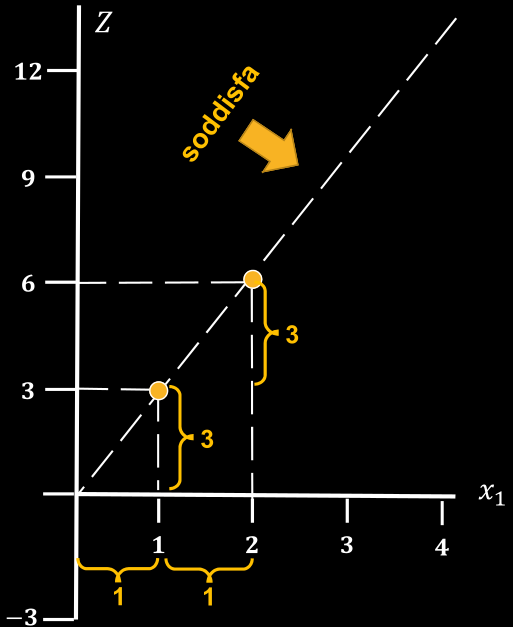
\includegraphics[scale=0.5]{Immagini/Proporzionalità1.png}
    \end{center}
\end{minipage}

\subsubsection{Esempio 2}
\begin{minipage}[t]{0.45\textwidth}
    L'immagine a destra mostra una situazione simile ma con un "costo di inizializzazione" (l'intercetta a $-1$ sull'asse verticale). 
    
    Questo introduce un elemento non lineare (affine, più precisamente), poiché il rapporto tra l'incremento di $Z$ e l'incremento di $x_1$ non è più costante rispetto all'origine. 
\end{minipage}
\hfill
\begin{minipage}[t]{0.45\textwidth}
    \vspace{0pt}
    \begin{center}
        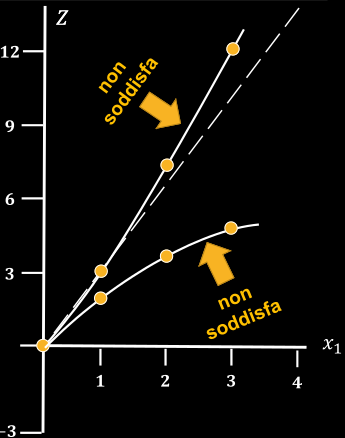
\includegraphics[scale=0.75]{Immagini/Proporzionalità 2.png}
    \end{center}
\end{minipage}

\newpage
\subsection{Assunzione di Additività}
\subsubsection{Definizione semplificata}
Ogni funzione è la somma dei contributi delle variabili decisionali

\subsubsection{Definizione matematica}
In un problema di programmazione lineare, il valore assunto da ogni funzione, sia essa \textbf{funzione obiettivo} o vincolo, è dato dalla somma dei contributi individuali delle rispettive attività

\subsubsection{Esempio}
\begin{center}
    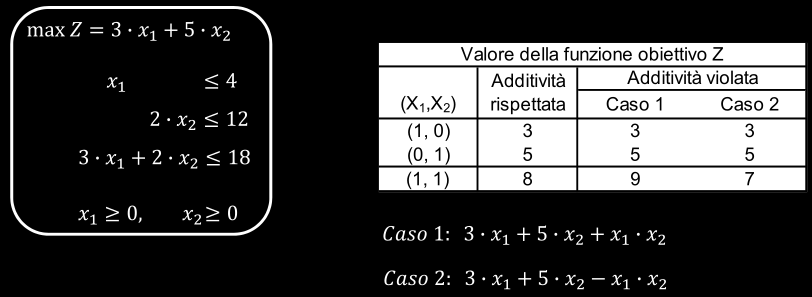
\includegraphics[scale=0.65]{Immagini/Additività.png}
\end{center}

\subsection{Assunzione di Divisibilità}
Le variabili decisionali in un programma di programmazione lineare sono libere di assumere qualsiasi valore, inclusi valori non interi che soddisfino i vincoli funzionali ed i vincoli di non negatività ( in altri termini, le variabili continue).

In alcune condizioni può accadere che le variabili decisionali non possano che assumere valori interi (non è possibile costruire un quarto di finiestra, non è possibile produrre 21.45 porte finestra).

In questi casi si parla di problema di programmazione lineare intera o a numeri interi

\subsection{Assunzione di Certezza}
Il valore assegnato ad ogni parametro di un problema di programmazione lineare è assunto essere non con certezza e costante

\newpage
\section{Soluzione Grafica}
\subsection{Cosa è?}
Per risolvere i problemi di programmazione lineare, possiamo adottare una procedura grafica, determinando i valori delle variabili decisionali $x_1,x_2$ che rispettano i vincoli, ed al tempo stesso rendendo massimo il valore $Z$ della funzione obiettivo.

La soluzione grafica si compone di:
\begin{itemize}
    \item Disegno della regione ammissibile
    \item Determinazione dell'ottimo
\end{itemize}

\subsection{Vincoli di Uguaglianza}
I vincoli $g_i(x)$ possono essere:
\begin{itemize}
    \item \textbf{Rette:} $g_i(x)=0$
    
    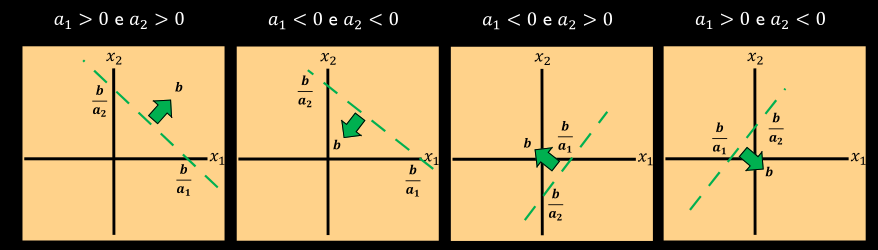
\includegraphics[scale=0.5]{Immagini/Rette.png}

    \item \textbf{Semipiani:} $g_i(x) \leq 0$
\end{itemize}

\subsubsection{Come rappresentiamo un semipiano?}
\begin{enumerate}
    \item Disegnamo la retta associata $(a_1 \cdot x_1 + a_2 \cdot x_2 \leq b)$
    \item Scegliamo un punto non appartenente a tale retta
    \begin{itemize}
        \item Se il punto verifica la disuguaglianza allora scegliamo il semipiano che lo contiene
        \item Altrimenti scegliamo l'altro semipiano
    \end{itemize}
\end{enumerate}

\begin{center}
    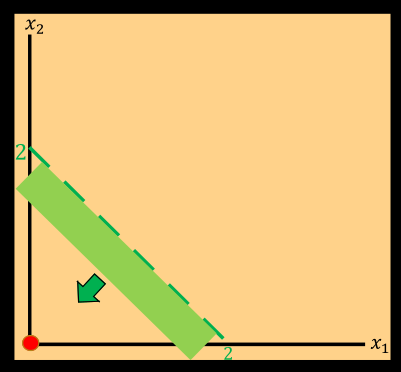
\includegraphics[scale=0.5]{Immagini/Semipiano.png}
\end{center}

\newpage
\subsection{Vincoli funzionali di $\leq$}
In maniera generalizzata, possiamo pensare che un problema di programmazione lineare è formulato in questo modo:

\begin{center}
    \[
    \setlength{\arraycolsep}{3pt}
    \begin{array}{l c c c c c c c l}
        \max Z = & c_1 \cdot x_1 & + & c_2 \cdot x_2 & + & \dots & + & c_n \cdot x_n & \\
        [1.5ex]
        & a_{11} \cdot x_1 & + & a_{12} \cdot x_2 & + & \dots & + & a_{1n} \cdot x_n & \leq b_1 \\
        [1ex]
        & a_{21} \cdot x_1 & + & a_{22} \cdot x_2 & + & \dots & + & a_{2n} \cdot x_n & \leq b_2 \\
        [1ex]
        & \dots \dots & + & \dots \dots & + & \dots & + & \dots \dots & \leq \dots \\
        [1ex]
        & a_{m1} \cdot x_1 & + & a_{m2} \cdot x_2 & + & \dots & + & a_{mn} \cdot x_n & \leq b_m \\
        [1.5ex]
        & \multicolumn{8}{l}{x_1 \geq 0, x_2 \geq 0, \dots, x_n \geq 0}
    \end{array}
    \]
\end{center}

Con :
\begin{itemize}
    \item Z funzione obiettivo
    \item $
    % \left. crea una delimitazione sinistra invisibile
    \left.
    \setlength{\arraycolsep}{3pt}
    \begin{array}{c c c c c c c l}
        a_{11} \cdot x_1 & + & a_{12} \cdot x_2 & + & \dots & + & a_{1n} \cdot x_n & \leq b_1 \\
        [1ex]
        a_{21} \cdot x_1 & + & a_{22} \cdot x_2 & + & \dots & + & a_{2n} \cdot x_n & \leq b_2 \\
        [1ex]
        \dots\dots & + & \dots\dots & + & \dots & + & \dots\dots & \leq \dots \\
        [1ex]
        a_{m1} \cdot x_1 & + & a_{m2} \cdot x_2 & + & \dots & + & a_{mn} \cdot x_n & \leq b_m 
    \end{array}
    % \right\} chiude il blocco con una graffa destra che si adatta all'altezza
    \right\} \text{ Vincoli funzionali}
    $
    \item $x_1 \geq 0,\ x_2\geq 0,\ x_3 \geq 0,\ \dots,\ x_m\geq 0$ vincoli di non negatività 
\end{itemize}

In particolare quindi:
\begin{itemize}
    \item $\mathbf{Z}$: Valore della misura di prestazione
    \item $\mathbf{x_j}$: Livello dell'attività $j$
    \item $\mathbf{c_j}$: Incremento del valore della misura di prestazione $Z$ corrispondente all'incremento di un'unità del valore dell'attività $x_j$
    \item $b_i$: Quantità di risorsa $"i"$ allocabile all'attività $x_j,\ j=1,\ \dots,\ n$
    \item $a_{ij}$: Quantità di risorsa $"i"$ consumata da ogni unitò di attività $x_j\ j=1,\ \dots,\ n$
\end{itemize}

\subsection{Vincoli di funzionalità di $\geq$ e $=$}
Generalizzando al caso con $n$ \textbf{variabili decisionali} ed $m$ \textbf{vincoli}, otteniamo la seguente formulazione di un \textbf{programmazione lineare}

\begin{itemize}
    \item \textbf{Funzione obiettivo:}: $opt\ Z$
    \item \textbf{Vincoli}: 
    $
    % \left. crea una delimitazione sinistra invisibile
    \left.
    \setlength{\arraycolsep}{3pt}
    \begin{array}{c c c c c c c l}
        a_{11} \cdot x_1 & + & a_{12} \cdot x_2 & + & \dots & + & a_{1n} \cdot x_n & \leq b_1 \\
        [1ex]
        a_{21} \cdot x_1 & + & a_{22} \cdot x_2 & + & \dots & + & a_{2n} \cdot x_n & \leq b_2 \\
        [1ex]
        \dots\dots & + & \dots\dots & + & \dots & + & \dots\dots & \leq \dots \\
        [1ex]
        a_{m1} \cdot x_1 & + & a_{m2} \cdot x_2 & + & \dots & + & a_{mn} \cdot x_n & \leq b_m 
    \end{array}
    % \right\} chiude il blocco con una graffa destra che si adatta all'altezza
    \right\} \text{ Vincoli funzionali}
    $
\end{itemize}

In questo caso quindi, siamo nel caso quale $x_2$ \textbf{non è vincolata} da nessun valore.

Inoltre, ogni vincolo $\geq$ e $=$ può essere riscritto nella seguente forma

\begin{itemize}
    \item $g_i(x) \geq b_i \to -g_i(x) \leq b_i$
    \item $g_i(x) = b_i \to 
    \begin{cases}
        g_i(x) \geq b_i \\
        g_i(x) \leq b_i    
    \end{cases}$
\end{itemize}

\section{Regione Ammissibile}
\subsection{Definizione}
La regione ammissibile $X$ è data dal soddisfacimento dei vari vincoli

$$
X = \{x \in \mathbb{R}^n : g_i(x) =   \left\{
        \begin{matrix}
        \geq \\
        = \\
        \leq
        \end{matrix}
        \right\}0,\ i=1,\ \dots,\ m
    \}
    \text{ con } g_i(x)=a_i^T-b_i
$$

dove $a \in \mathbb{R}^n. b\in\mathbb{R}^m$

\subsection{Proprietà della Regione Ammissibile}
La regione ammissibile, da un punto di vista geometrico, corrisponde ad un \textbf{poliedro convesso in } $\mathbf{R}^n$.

La regione ammissibile può essere limitata o illimitata

\begin{center}
    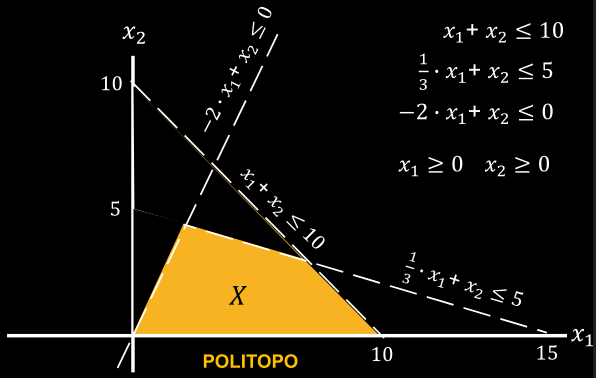
\includegraphics[scale=0.5]{Immagini/RA PL.png}
\end{center}

\subsection{Possibili soluzioni}
Si possono verificare 4 soluzioni:
\begin{itemize}
    \item Il problema di programmazione lineare \textbf{ammette una sola soluzione ottima in un vertice del poligono convesso} che delimita la regione ammissibile
    \item Il problema di programmazione lineare \textbf{ammette infinite soluzioni ottime in un lato del poligono commesso} che delimita la regione ammissibile se la direzione di decrescita è perpendicolare ad un lato del poligono
    \item Il problema di programmazione lineare \textbf{ammette infinite soluzioni} perchè la regione ammissibile è illimitata e la funzione obiettivo è illimitata superiormente (se è di massimizzazione) o inferiormente (se di minimizzazione)
    \item Il problema di programmazione \textbf{non ammette soluzione} perchè la regione ammissibile è vuota 
\end{itemize}

Per risolvere quindi un problema di programmazione lineare:
\begin{enumerate}
    \item Disegnare la regione ammissibile
    \item Cercare di massimizzare/minizzare la soluzione, riportando ciò che troviamo sul grafico
\end{enumerate}

        
    
    \part{Esercizi}

    \part{Laboratori}

\end{document}